\documentclass{article}

\renewcommand{\familydefault}{\sfdefault}  %serifenlose Schrift
\usepackage{helvet} % Schrift: Helvetica


\usepackage{graphicx,graphics,tikz}
\usepackage{amsmath}
\usepackage{amsthm}
\usepackage{amsfonts}
\usepackage{amssymb}
\usepackage{marvosym} % to be able to show male and female symbols with: \Female and \Male
\usepackage{gensymb}
\usepackage[graphics,tightpage,active]{preview}
\PreviewEnvironment{tikzpicture}
\newlength\imagewidth
\newlength\imagescale

\begin{document}

\pgfmathsetlength{\imagewidth}{10cm} % desired displayed width of image
\pgfmathsetlength{\imagescale}{\imagewidth/2000} % pixel width of image
% adjust scale of tikzpicture (and direction of y) such that pixel
% coordinates can be used for drawing overlays:
\usetikzlibrary{backgrounds}

\begin{tikzpicture}[x=\imagescale,y=-\imagescale]

\node at (0cm,0cm) {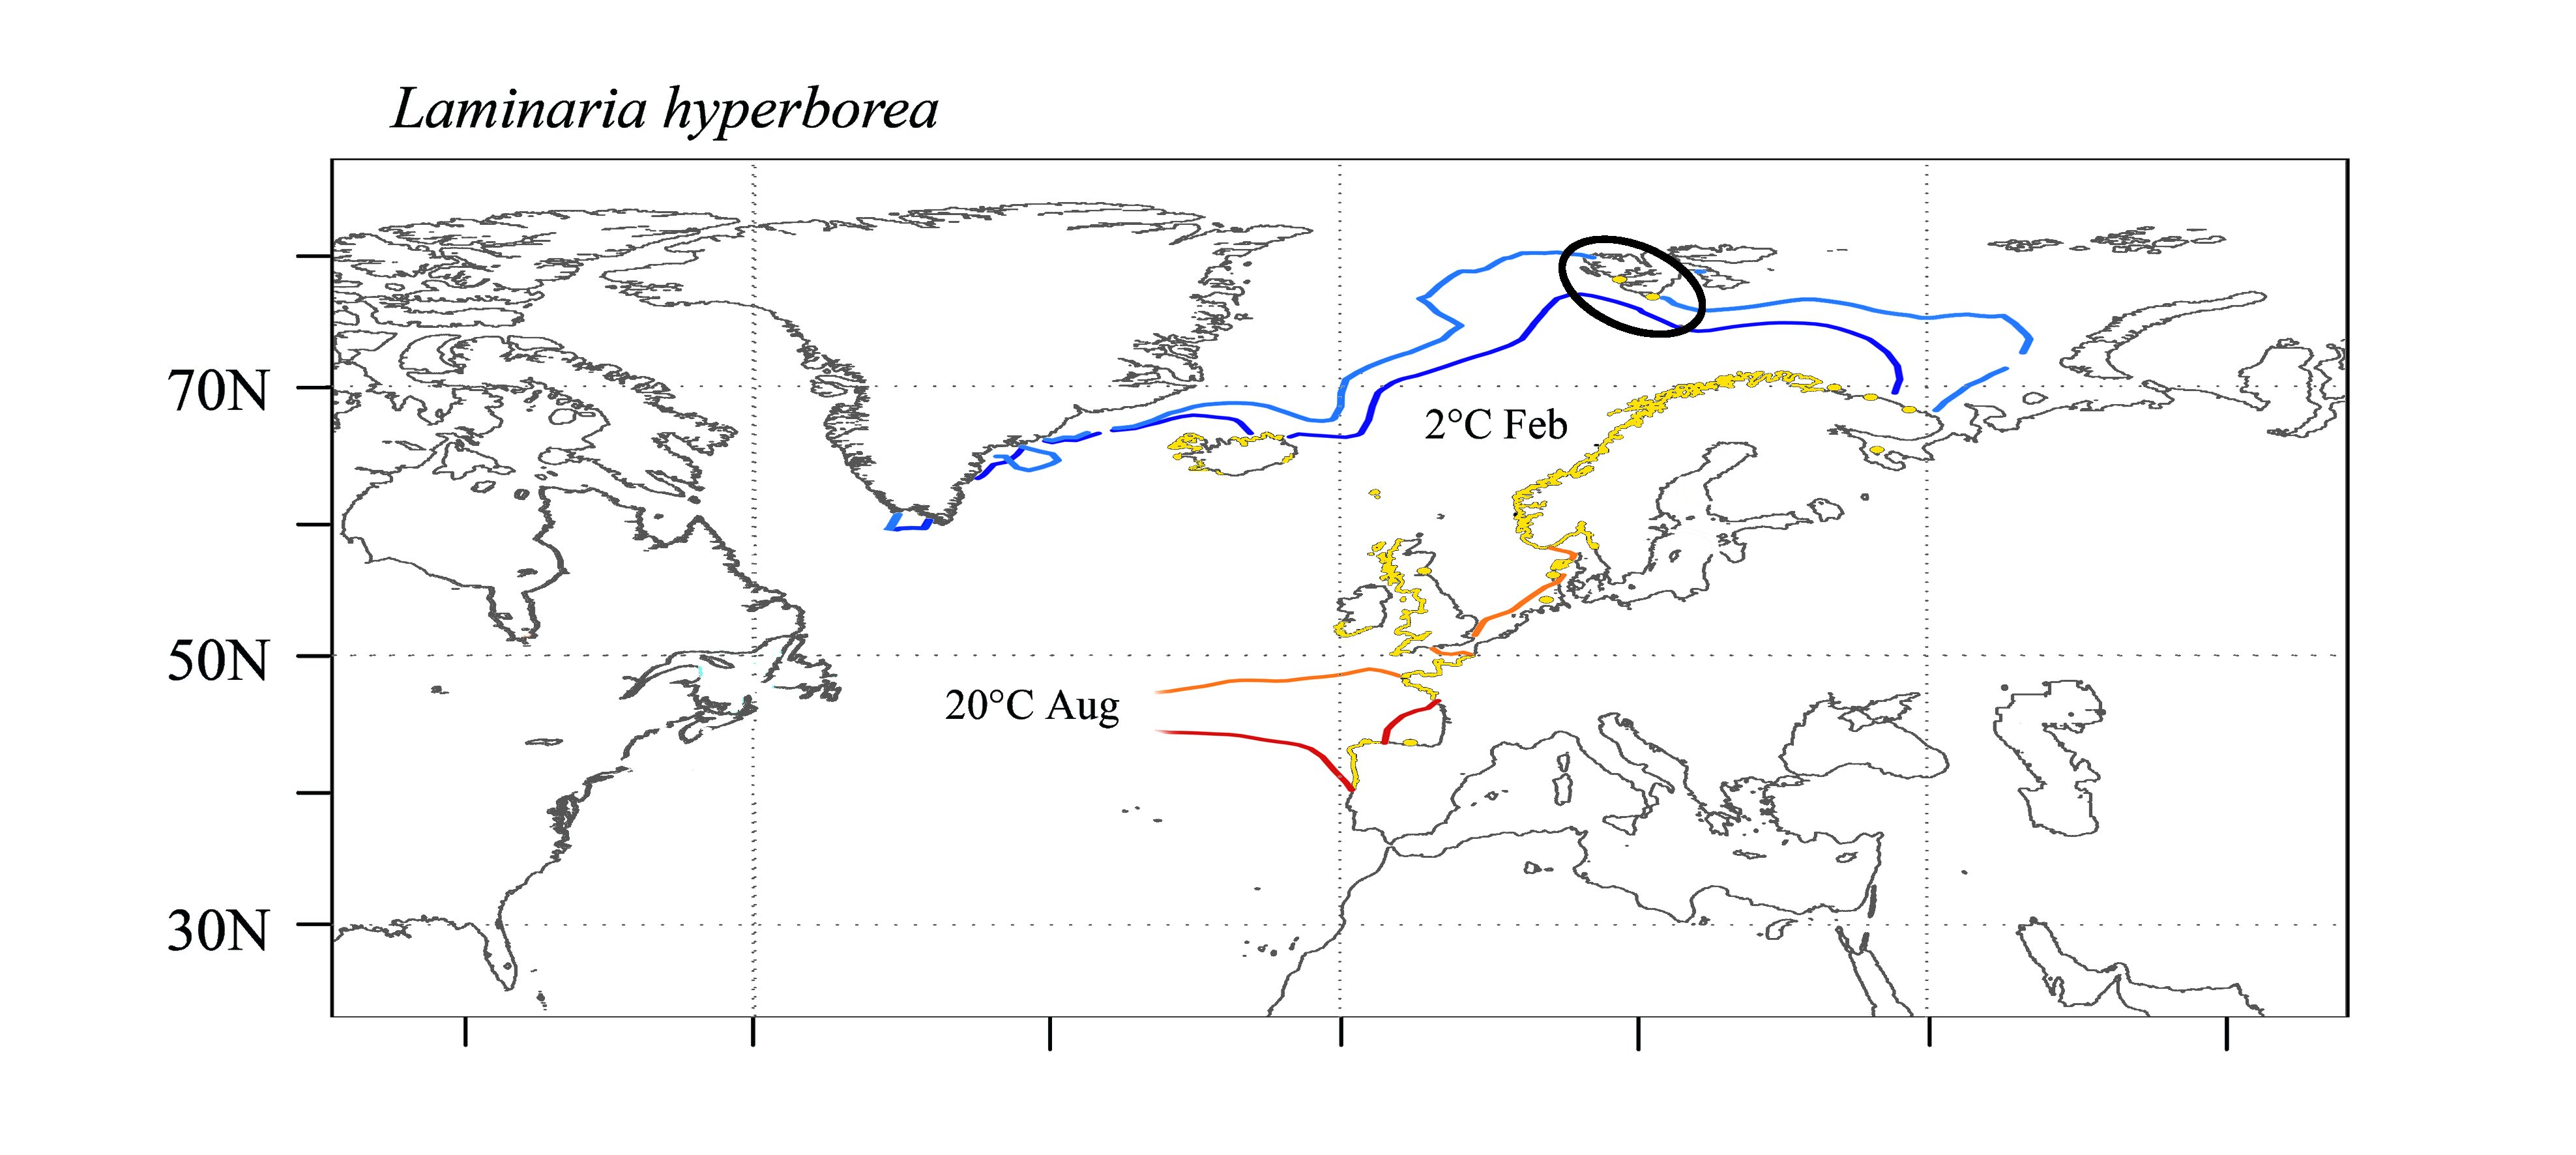
\includegraphics[width=12cm]{Figure3_Mueller_etal_BotaMar_adjusted.jpg}};
\node [text centered] at (2.2cm,1.75cm) {\scriptsize{Recent records}};


\node at (-3.45cm,0.65cm) {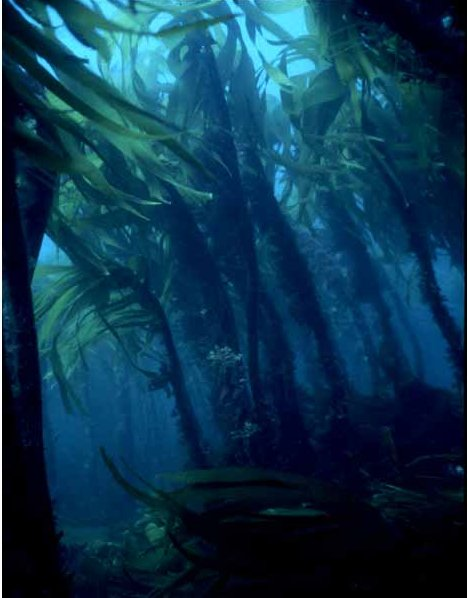
\includegraphics[width=2cm]{KeithHiscock_LaminariaHyperborea.jpg}};
\node [text centered,color=white,scale=0.7] at (-3.3cm,-0.4cm) {\scriptsize{Hiscock, K.}};
\end{tikzpicture}

\end{document}